% Options for packages loaded elsewhere
\PassOptionsToPackage{unicode}{hyperref}
\PassOptionsToPackage{hyphens}{url}
%
\documentclass[
  12pt,
]{article}
\usepackage{amsmath,amssymb}
\usepackage{lmodern}
\usepackage{iftex}
\ifPDFTeX
  \usepackage[T1]{fontenc}
  \usepackage[utf8]{inputenc}
  \usepackage{textcomp} % provide euro and other symbols
\else % if luatex or xetex
  \usepackage{unicode-math}
  \defaultfontfeatures{Scale=MatchLowercase}
  \defaultfontfeatures[\rmfamily]{Ligatures=TeX,Scale=1}
\fi
% Use upquote if available, for straight quotes in verbatim environments
\IfFileExists{upquote.sty}{\usepackage{upquote}}{}
\IfFileExists{microtype.sty}{% use microtype if available
  \usepackage[]{microtype}
  \UseMicrotypeSet[protrusion]{basicmath} % disable protrusion for tt fonts
}{}
\makeatletter
\@ifundefined{KOMAClassName}{% if non-KOMA class
  \IfFileExists{parskip.sty}{%
    \usepackage{parskip}
  }{% else
    \setlength{\parindent}{0pt}
    \setlength{\parskip}{6pt plus 2pt minus 1pt}}
}{% if KOMA class
  \KOMAoptions{parskip=half}}
\makeatother
\usepackage{xcolor}
\IfFileExists{xurl.sty}{\usepackage{xurl}}{} % add URL line breaks if available
\IfFileExists{bookmark.sty}{\usepackage{bookmark}}{\usepackage{hyperref}}
\hypersetup{
  pdftitle={Learning with misspecified models: Overconfidence and Stereotypes},
  pdfauthor={Jimena Galindo},
  hidelinks,
  pdfcreator={LaTeX via pandoc}}
\urlstyle{same} % disable monospaced font for URLs
\usepackage[margin=2.5cm]{geometry}
\usepackage{graphicx}
\makeatletter
\def\maxwidth{\ifdim\Gin@nat@width>\linewidth\linewidth\else\Gin@nat@width\fi}
\def\maxheight{\ifdim\Gin@nat@height>\textheight\textheight\else\Gin@nat@height\fi}
\makeatother
% Scale images if necessary, so that they will not overflow the page
% margins by default, and it is still possible to overwrite the defaults
% using explicit options in \includegraphics[width, height, ...]{}
\setkeys{Gin}{width=\maxwidth,height=\maxheight,keepaspectratio}
% Set default figure placement to htbp
\makeatletter
\def\fps@figure{htbp}
\makeatother
\setlength{\emergencystretch}{3em} % prevent overfull lines
\providecommand{\tightlist}{%
  \setlength{\itemsep}{0pt}\setlength{\parskip}{0pt}}
\setcounter{secnumdepth}{5}

\setlength{\parindent}{25pt}
\setlength{\parskip}{0pt}
\setlength{\skip\footins}{0.25cm} % margin before footnotes
\definecolor{myblue}{RGB}{31, 61, 122}
\definecolor{mypink}{RGB}{204, 0, 82}
\newtheorem{assumption}{Assumption}
\newtheorem{proposition}{Proposition} % Use the 'proposition' counter for numbering

\newcommand{\EE}[1]{\mathbb{E}\left[#1\right]}
\newcommand{\PP}[1]{\mathbb{P}\left(#1\right)}
\newcommand{\CP}[2]{\mathbb{P}\left(#1 \,| \, #2 \right)}
\newcommand{\CE}[2]{\mathbb{E}\left[#1\,|\,#2 \right]}
\usepackage[bottom]{footmisc}
\usepackage[doublespacing]{setspace}
\usepackage[normal]{caption}
\usepackage{dsfont}
\usepackage{booktabs}
\usepackage{makecell}
\usepackage{hyperref}
\ifLuaTeX
  \usepackage{selnolig}  % disable illegal ligatures
\fi
\usepackage[]{natbib}
\bibliographystyle{plainnat}

\title{Learning with misspecified models: Overconfidence and
Stereotypes}
\author{Jimena Galindo}
\date{October 07, 2023}

\begin{document}
\maketitle
\begin{abstract}
TBW
\end{abstract}

\hypertarget{introduction}{%
\section{Introduction}\label{introduction}}

\hypertarget{related-literature}{%
\subsection{Related literature}\label{related-literature}}

\hypertarget{theoretical-framework}{%
\section{Theoretical Framework}\label{theoretical-framework}}

I consider multiple theories of belief updating that have been proposed
in the literature and that are able to rationalize the prevalence of
misspecified beliefs. I focus on two different frameworks and develop a
unifying example that allows me to compare the predictions of all the
theories. In this section, I outline the theories within each of the
frameworks.

\hypertarget{framework-1}{%
\subsection{Framework 1}\label{framework-1}}

An agent is of type \(\theta \in \Theta\) and faces an unknown exogenous
state \(\omega\) drawn from some density \(f\) over \(\Omega\). The
agent knows the distribution of \(\omega\) but not its realized value.
His prior belief about his type is \(p_0(\theta)\) and his belief about
the state, \(p_0(\omega)\), coincides with the true distribution. Let
the agent's true type be \(\theta^{*}\), and the realized state be
\(\omega^{*}\).

An agent has a \emph{misspecified} belief if the prior assigns
probability zero to their true type. Furthermore, the agent is
\emph{dogmatic} if he holds a degenerate belief that places probability
one on being a particular type, \(\hat{\theta}\). An agent can be
dogmatic and misspecified. If the agent is both,
\(\hat{\theta} \neq \theta^*\) and \(p_0(\hat{\theta}) = 1\).

The agent chooses an action \(a\in A\) and observes a noisy outcome
\(h\in H\). The outcome is a function of the agent's type, the state,
and the action. In particular
\(h = h(\theta^*, \omega^*, a) + \varepsilon\) with \(h(\cdot)\)
increasing in both \(\theta^*\) and \(\omega^*\), and such that
conditional on a pair of parameters \((\theta, \omega)\), there is a
unique optimal action. \(\varepsilon\sim N(0, \sigma)\) is noise in the
output.

After observing the outcome, the agent updates his beliefs about
\(\theta\) and \(\omega\) using some algorithm and moves on to the next
period. He repeats this process infinitely many times. I make the
simplifying assumption that the agent is myopic and chooses the action
that maximizes the payoff in each period. This assumption simplifies the
analysis and plays a role in whether an agent who updates their beliefs
using Bayes rule would learn the truth or not. The behavior of a
forward-looking agent is discussed in the conclusion.

A key notion in this setting is that of a self-defeating
equilibrium\footnote{This notion is an adaptation of the Berk-Nash equilibrium in 
@Esponda2016 to this setting with only one agent}. A
\emph{self-defeating equilibrium} is a belief and action pair such that
the agent's belief about their type is misspecified and the outcome
generated by the action is consistent with the misspecified belief. This
means that the average outcome under the true type and the true state
equals the average output the agent expects under the misspecified
belief. The agent's belief is said to be \emph{stable} when this
happens.

Within this framework, I consider two nested theories of belief
updating: the first one is a dogmatic modeler from \citet{Heidhues2018},
The second one is a switcher, as in \citet{Ba2023}. The dogmatic modeler
can be seen as a switcher with an infinitely sticky initial belief and
this is the sense in which the two are nested. Both theories produce
different predictions about the agent's behavior. I discuss both in what
follows.

\hypertarget{the-dogmatic-modeler}{%
\subsubsection{The Dogmatic Modeler}\label{the-dogmatic-modeler}}

A dogmatic agent does not update their beliefs about \(\theta\),
instead, he holds a degenerate belief that places probability on
\(\hat{\theta}\), which is potentially misspecified. In this case, no
matter how much information he gathers against being of type
\(\hat{\theta}\), he will not update his beliefs about \(\theta\). Any
discrepancies between the observed outcomes and his believed type are
incorporated using the Bayes rule to update their beliefs about
\(\omega\). \citet{Heidhues2018} show that, under certain assumptions on
the per-period utility,\footnote{The assumptions are that 
$u$ is twice continuously differentiable with: (i)$u_{ee}<0$ and $u_e(\underline{e} \theta, \omega)>0>u_e(\Bar{e}, \theta, \omega)$, 
(ii) $u_{\theta}, u_{\omega}>0$ and (iii) $u_{e\theta}<0$ and $u_{e\omega}>0$. The direction of the derivatives is a normalization
and the results would hold even when the signs are reversed.} a dogmatic
modeler will inevitably fall into a self-defeating equilibrium. The
equilibrium will be such that the outcomes they observe reinforce their
belief on \(\omega\) in such a way that as \(t\to\infty\) the agent will
be sure that the state is some \(\omega^{'}\) consistent with their
believed type and the observed data. In other words, they will be in a
self-defeating equilibrium with a stable belief that places probability
one on the incorrect parameters \((\hat{\theta}, \omega_{\infty})\)

The mechanism by which the dogmatic agent falls into the self-defeating
equilibrium is the following: Suppose the agent holds the misspecified
belief that they are type \(\hat{\theta}>\theta^*\). For any prior over
\(\omega\), the agent will be disappointed by the outcome. He expected a
gain of \(h(\hat{\theta}, \mathbb{E}(\omega), a)\) but instead observes
\(h(\hat{\theta}, \omega^*, a)\). There are two possible sources for the
disappointment, the first is that the realized state is lower than the
expected state. The second source is that the agent is of type
\(\theta^*\) and therefore, for all possible states, his gain will be
lower than what he expected. Because the agent is dogmatic, he will not
update his beliefs about \(\theta\) and as a consequence will attribute
the disappointment to the state being lower than expected. He will
continue to update in this way until he converges to a belief about
\(\omega\) that is stable. Such a belief will explain the observed
utility perfectly and allow the agent to rationalize his dogmatic belief
about \(\theta\). Under the assumptions of \citet{Heidhues2018}, there
is a unique value of \(\omega\) at which the belief is stable, I will
refer to such value as \(\omega_\infty\). This mechanism is further
illustrated in Example 1.

\textbf{Example 1: } \emph{Set \(A = \Omega\) and \(H = [0, \infty)\)
and consider a student with intrinsic ability \(\theta^*\geq 0\) who
faces a grading procedure \(\omega^*\) that is unknown to them. However,
they know that a higher \(\omega^*\) is more likely to yield a higher
grade. In particular, assume the grade is given by
\((\theta^*+a)\omega^*\).}

\emph{The student must choose an effort level \(a\), which determines
their grade. For whatever the chosen effort level, the agent must pay a
cost \(c(a) = \frac{1}{2}a^2\). And he repeats this process for
infinitely many periods. Assume also that the student's prior is such
that \(mathbb{E}[\omega]= \omega^*\) and he is dogmatic about being of
type \(\hat{\theta}>\theta^*\).
\footnote{The example is illustrated for an overconfident agent but the results are symmetric for a digmatic agent who initially 
places probability one on some $\tilde{\theta}<\theta^*$.} Therefore,
the student's payoff in period \(t\) is given by }

\begin{equation}
u_t(a_t; \theta^*, \omega^*) = (\theta^*+a_t)\omega^* - \frac{1}{2}a^2 + \varepsilon_t
\end{equation}

\emph{Under this specification, the myopic optimal effort level is
\(a_t^* = \omega^*\). Nonetheless, because the agent does not know
\(\omega^*\), he will choose \(a_t = \mathbb{E}_t(\omega)\) where the
expectation is taken with respect to the agent's belief at the beginning
of period \(t\). If he does not revise his effort choice for \(k\)
periods, he will receive an average utility of
\((\theta^*+a_t^*)\omega^* - \frac{1}{2}a_t^{*2}\) but he was expecting
an average utility of
\((\hat{\theta}\theta+a_t^*)\omega^* - \frac{1}{2}a_t^{*2}\). In
response, he will apply Bayes rule to update his beliefs about
\(\omega\) to get the posterior belief with
\(\mathbb{E}_{t+k}[\omega] = \frac{(\theta^{*} + \omega^{*})\omega^{*}}{\hat{\theta} + \omega^{*}}\)
which is lower than the initial belief. This will cause the agent to
choose a lower effort at \(t+k\). As a result, he will again receive an
average utility that is lower than what he expected which will cause his
belief to drift further down. This process will continue until the
average utility equals his expected utility under the dogmatic belief
that assigns probability 1 to \(\hat{\theta}\). At that point, the
student will have reached a self-defeating equilibrium and he will
continue to choose sub-optimal effort forever. }

Although the model of a dogmatic modeler rationalizes the prevalence of
overconfident (underconfident) beliefs, the assumption that the agent
has a degenerate belief and no mechanism through which he can update
such belief is very restrictive. An alternative approach is proposed by
\citet{Ba2023}. She proposes an extension of the dogmatic agent who is
able to jump from one dogmatic belief to another. By doing so, the agent
might end up being dogmatic and correctly specified.

\hypertarget{the-switcher}{%
\subsubsection{The Switcher}\label{the-switcher}}

An agent is a \emph{switcher} if they behave as a dogmatic, but is
willing to entertain the possibility that they are of a different type.
In particular, when they start off as a misspecified dogmatic, they are
willing to switch to a different dogmatic belief if the data is
convincing enough. Their prior is still degenerate and assigns
probability one to a particular type, and zero to all other types. This
means that a Bayesian update on \(\theta\) does not change their beliefs
about the type. However, they are willing to entertain two such beliefs
and have a mechanism by which they decide which belief to adopt at any
period \(t\).

In order to abandon their initial dogmatic belief, the agent needs to
observe a sequence of outcomes that are sufficiently unlikely to have
happened if they were of the type they initially believed. In order to
evaluate if the evidence is convincing enough, they keep track of the
likelihood that each of the possible types generated the data. If the
likelihood ratio is sufficiently large, the agent will switch to the
alternative and behave as if they are dogmatic about the new type.

In particular, for an agent that starts with a dogmatic belief that they
are of type \(\hat{\theta}\) but is willing to consider the alternative
explanation that they are of type \(\tilde{\theta}\), the agent will
switch to the alternative if:

\[\frac{p[h^t|\tilde{\theta}]}{p[h^t|\hat{\theta}]} > \alpha\geq 1\]

Where \(h^t\) is the history of outcomes up to time \(t\) and \(\alpha\)
is the switching threshold. By keeping track of the likelihood ratio,
the agent can perform a \emph{Bayesian hypothesis test} and adopt the
Dogmatic belief that best fits the
data.\footnote{In a related problem @Schwarstein2021 proposes a similar updating procedure which relies on the Bayesian 
hypothesis test. However, in their model there is a sender who optimally chooses to propose a model that fits the data}
Notice that if \(\alpha \to \infty\), the behavior of the switcher will
be indistinguishable from that of the Dogmatic modeler. In this sense,
the switcher is a generalization of the dogmatic type.

By allowing the agent to keep track of the likelihoods and switching to
an alternative type, the switcher can avoid the self-confirming
equilibrium. However, if the prior belief on \(omega\) is sufficiently
tight around a self-defeating equilibrium, the switcher might look
identical to the dogmatic even in a case where \(\alpha\) is not too
large. This happens because under the agent's prior, the likelihood
ratio is unlikely to grow as fast as it is needed to escape the
self-defeating equilibrium. In such situations, we say that the
misspecified belief is persistent.

\hypertarget{framework-2}{%
\subsection{Framework 2}\label{framework-2}}

As in framework 1, the agent is of some type \(\theta^* \in \Theta\) and
the state is \(\omega \sim F(\Omega)\). In this case, the agent chooses
an action \(a\in A\) and observes a binary outcome that is either a
success or a failure. Denote the outcome by \(o \in {s,f}\). The
probability of observing a success is increasing in \(\theta^*\) and in
\(\omega\). Whenever the agent observes a success, he gets a payoff
\(v>0\) and whenever the outcome is a failure, the payoff is 0. In
addition, the probability of success is such that for each state, there
is a unique optimal action that maximizes the agent's expected payoff.
Therefore, the probability of success can be seen as a monotone
transformation of the utility from Framework 1.

I focus on two nested theories that have been widely studied within this
framework: Full Bayesian updating and self-serving attribution bias. I
explain each of these classical models of belief updating in what
follows

\hypertarget{the-bayesian}{%
\subsubsection{The Bayesian}\label{the-bayesian}}

A Bayesian agent simultaneously updates their beliefs about \(\theta\)
and \(\omega\) by using Bayes' rule. The posterior at period t+1 about
\(\theta\) after observing a history of outcomes \(h^t\) is given by: \[
p_{t+1}(\theta, \omega| h^t) = \frac{p[h^t|\theta, \omega]p_t(\theta, \omega)}{\sum_{(\theta', \omega')}p[h^t|\theta', \omega']p_t(\theta', \omega')}
\]

Where \(p_{t}\) is the belief at the start of period \(t+1\). The update
is symmetric for \(\omega\).

Bayesian agents choose the effort level that maximizes their expected
flow payoff by taking expectations over their prior beliefs about
\(\theta\) and \(\omega\). Since agents are myopic, even though all the
parameters could be identified with enough variation in choices.
Although the Bayesian agent is the closest to a fully rational agent
discussed here, they might not learn their true type. This happens
because, by being myopic, they do not internalize the tradeoff between
flow payoff and learning. This can result in too little experimentation
to learn their true type. An alternative to this approach is given by
\citet{Hestermann2021} and is discussed in the concluding remarks.

Also notice that if a fully Bayesian agent has a dogmatic prior, they
will never update their beliefs about the parameter that they are
dogmatic about. This will imply that they are prone to the same types of
errors as the dogmatic modeler in framework 1.

\hypertarget{the-self-serving-updater}{%
\subsubsection{The Self-Serving
Updater}\label{the-self-serving-updater}}

A self-serving Bayesian is an agent who uses a biased version of Bayes
rule to update their beliefs. They will update their beliefs about the
state \(\omega\) and his type \(\theta\) simultaneously by
over-attributing successes to a high value of \(\theta\) and
under-estimating the role of higher \(\omega\). Similarly, he will
attribute failure to a low state to a greater degree than an unbiased
agent would. To model the self-serving attribution bias, I take the
approach of \citet{benjamin2019}, where the posterior odds are given by:

\[
p_{t+1}(\theta, \omega| h^t) = \frac{p[h^t|\theta, \omega]^{c(\theta, \omega, o_t)}p_t(\theta, \omega)}{\sum_{(\theta', \omega')}p[h^t|\theta', \omega']^{c(\theta, \omega, o_t)}p_t(\theta', \omega')}
\]

with
\(c(\theta_H, \omega, o)<c(\theta_M, \omega, o)<c(\theta_L, \omega, o)\leq 1\)
and
\(c(\theta, \omega_L, o)<c(\theta, \omega_M, o)<c(\theta, \omega_H, o)\leq 1\).

This formulation of the bias means that the agent will over-attribute
successes to a high type and under-attribute them to a low type. Whereas
they will over-attribute failures to a low state and under-attribute
them to a high state. The parameter \(c\) determines the degree of bias
and the restriction on the order ensures that the model is still
falsifiable.

\hypertarget{a-unifying-example}{%
\section{A Unifying Example}\label{a-unifying-example}}

In order to compare the predictions of the theories discussed above, I
develop a unifying example that allows me to isolate the forces behind
each of the theories. The example is a modification of the one in
\citet{Heidhues2018} and is adapeted to be easier to implement in the
lab.

The agent can be of one of 3 types:
\(\theta \in \{\theta_L, \theta_M, \theta_H\}\) with
\(\theta_H > \theta_M > \theta_L\). They face an unknown exogenous
success rate \(\omega \in \{\omega_L, \omega_M, \omega_H\}\) with
\(\omega_H>\omega_M>\omega_L\). Each of the values of \(\omega\) is
realized with equal probability. The agent knows the distribution of
\(\omega\) but not its realized value.

Denote the true type by \(\theta^*\) and the true state by \(\omega^*\).
The agent holds some prior belief about \(\theta\)
\footnote{which is potentially misspecified as in the dogmatic and switcher cases discussed above}
and chooses a binary gamble \(e in \{e_L, e_M, e_H\}\). The agent
observes whether the gamble is a success or a failure and gets a payoff
of \(1\) and if it is a success; they get \(0\) otherwise.

The probability of success is increasing in both \(\theta\) and
\(\omega\) and is fully described by the following table:

\begin{table}[htbp]

\begin{tabular}{ c|c|c|c|}
  
  \multicolumn{1}{c}{} & \multicolumn{1}{c}{$\omega_H$} & \multicolumn{1}{c}{$\omega_M$} & \multicolumn{1}{c}{$\omega_L$}\\
  \cline{2-4}
  $e_H$ & 50 & 20 & 2 \\
  \cline{2-4}
  $e_M$ & 45 & 30 & 7 \\
  \cline{2-4}
  $e_L$ & 40 & 25 & 20 \\

  \cline{2-4}
  \multicolumn{1}{c}{} & \multicolumn{1}{c}{} & \multicolumn{1}{c}{$\theta_L$} & \multicolumn{1}{c}{}\\
\end{tabular}
\hspace{.3cm} 
\begin{tabular}{ c|c|c|c|}
  
  \multicolumn{1}{c}{} & \multicolumn{1}{c}{$\omega_H$} & \multicolumn{1}{c}{$\omega_M$} & \multicolumn{1}{c}{$\omega_L$}\\
  \cline{2-4}
  $e_H$ & 80 & 50 & 5 \\
  \cline{2-4}
  $e_M$ & 69 & 65 & 30 \\
  \cline{2-4}
  $e_L$ & 65 & 45 & 40 \\
  \cline{2-4}
  \multicolumn{1}{c}{} & \multicolumn{1}{c}{} & \multicolumn{1}{c}{$\theta_M$} & \multicolumn{1}{c}{}\\
\end{tabular}
\hspace{.3cm} 
\begin{tabular}{ c|c|c|c|}
  
  \multicolumn{1}{c}{} & \multicolumn{1}{c}{$\omega_H$} & \multicolumn{1}{c}{$\omega_M$} & \multicolumn{1}{c}{$\omega_L$}\\
  \cline{2-4}
  $e_H$ & 98 & 65 & 25 \\
  \cline{2-4}
  $e_M$ & 80 & 69 & 35 \\
  \cline{2-4}
  $e_L$ & 75 & 55 & 45 \\
  \cline{2-4}
  \multicolumn{1}{c}{} & \multicolumn{1}{c}{} & \multicolumn{1}{c}{$\theta_H$} & \multicolumn{1}{c}{}\\
\end{tabular}

\caption{Probability of success for each type, gamble and effort level}
\label{tab:table1}
\end{table}

Conditional on a type, the agent's flow payoff is maximized by choosing
the gamble that matches the state. For example, if the value of
\(\omega\) is \(\omega_H\), the agent's flow payoff is maximized by
choosing \(e_H\) and if the state is \(\omega_L\) the flow payoff is
maximized by choosing gamble \(e_L\), regardless of the value of
\(\theta\). The agent myopically chooses gambles every period to
maximize the flow payoff for \(T<\infty\) periods.

After observing the outcome of each gamble, the agent updates their
beliefs using some procedure and moves on to the next period.

Notice that both \(\theta\) and \(\omega\) can be identified from the
outcomes if enough variation in the effort choices exists. This can be
seen by confirming that there is no pair of \(\theta\) and \(\omega\)
such that the probability of success is the same for all effort choices.
Thus, by changing the effort choice, the agent can learn both their type
and the state if they observe enough outcomes.

In this example, for an agent with a dogmatic belief about their type, a
self-defeating equilibrium is one in which the agent chooses an effort
level that, under the true \(\theta\), yields a frequency of success
that is consistent with the agent's misspecified belief. That is
\(P[\text{sucess}|\theta^*, e^*] = P[\text{sucess}|\hat{\theta}, e^*]\)
where \(e^*\) is the agent's myopic optimal choice.

In the data-generating process described above, there are five such
equilibria. For example, if the agent is of type \(\theta_M\) but
mistakenly believes that he is of type \(\hat{\theta}=\theta_H\) and the
and \(\omega^* = \omega_M\), when the effort chosen is \(e_L\), the
agent will observe a success with 45\% chance. Because the agent
dogmatically believes that their type is high, they will erroneously
conclude that the rate is \(\omega_L\). Under this belief, the optimal
action is \(e_L\) which will continue to generate successes with \(45%
\) probability, further reinforcing the incorrect belief. By doing so,
the agent forgoes the payoff from gamble \(e_M\) which would yield a
success with \(65\%\) chance.

By including self-confirming equilibria, the example captures the forces
from each of the updating mechanisms discussed in the previous section
and allows for the comparison of the main forces behind the theories.
For realizations of \((\theta, \omega)\) for which there are
self-confirming equilibria, the dogmatic agent will fall into the trap
whereas the switcher will be able to escape it. Similarly, an agent with
self-attribution bias will update their beliefs differently from an
unbiased Bayesian, leading them to choose different gambles. I exploit
such cases in order to test which model is a better fit for how subjects
behave in a laboratory experiment.
\footnote{because the setting does not match that of Heidhues et al. [2018], there will be situationf for which the theory 
does not provide a prediction. If such cases arise in the lab, they will not be used for the analysis. However, whether a misspecified 
belief persists or not for the switcher, depends highly on the realized history of signals that he gets.}
In what follows I explain the details of how this example was
implemented in the lab.

\hypertarget{experimental-design}{%
\section{Experimental Design}\label{experimental-design}}

I recruited undergraduate subjects from the CESS lab at NYU who
participated in an in-person experiment. Sessions lasted approximately
45 minutes and subjects earned an average payment of \(\$22.6\). The
experiment was programmed using oTree \citep{chen2016otree}.

The experiment consisted of 2 treatments: the \emph{ego-relevant}
condition and the \emph{stereotype} condition. Subjects participated in
only one of the treatments. All subjects within a session participated
in the same treatment and the first 4 treatments were assigned the
ego-relevant condition; the rest were assigned to the stereotype
treatment. The tasks were identical across treatments, except for
parameter \(\theta\). In the ego-relevant condition \(\theta\) is the
subject's own performance in a quiz, while in the stereotype condition,
it is the performance of a randomly selected subject from another
session.

The experiment had 3 parts. In Part 1 subjects had 2 minutes to answer
as many multiple-choice questions as they could from a 20-question quiz.
They did this for quizzes on 6 different topics. The topics were: Math,
Verbal Reasoning, Pop-culture and Art, Science and Technology, US
Geography, and Sports and Video Games. In this part, they did not know
how many questions were available and they were given no feedback.

After taking all 6 quizzes, they proceeded to part 2 where they were
asked to guess their score on each of them. In the stereotype treatment
they were additionally asked to guess the score of a randomly drawn
participant from a previous session. All they knew about the other
participant was their gender identity and whether they were US nationals
or not. For each guess, they had three score options: Low-Score (5 or
fewer correct answers), Mid-Score (between 6 and 15 correct answers),
High-Score (16 or more). Each of the score categories corresponded to
\(\theta_L\), \(\theta_M\), and \(\theta_H\) respectively. They were
also asked to say how confident they felt about their choices. They had
4 possible answers: ``it was a random guess'', ``there is another
equally likely score'', ``I am pretty sure'', ``I am completely sure''.
These 4 answers are mapped to priors that place probabilities .33, .50,
.75, and 1 to the chosen type. The remaining probability is split
equally among the other two types. Questions in Part 2 were not
incentivized, but subjects were told that providing an accurate answer
would increase their chances of earning more money in the last part of
the experiment.

The purpose of Part 2 is to classify subjects into overconfident,
underconfident and correctly specified. If a subject guesses their score
to be in a higher (lower) category than their true score, they are
overconfident (underconfident); if they guess their score to be in the
same category as their true score, they are correctly specified. This
classification is done for each of the 6 topics separately.

Finally, in Part 3, subjects completed a belief updating task for each
of the quizzes. Before starting the task they were reminded of their
guess for the score. In the ego-relevant treatment, they were reminded
of their guess about themselves and in the stereotype treatment they
were reminded of their guess about the other participant. In the
stereotype treatment, they were also reminded of the characteristics of
the other participant.

For one topic at a time and in random order, they were presented with
the three gambles from the example above and were asked to choose one of
them. The probability of success was determined by their own score in
the ego-relevant condition, and by the score of the other participant in
the stereotype condition. Subjects had access to the three probability
tables in the printout of the instructions at all times and the meaning
of each cell was explained in detail.

In the interphase, they had to choose which of the 3 tables they wanted
to see before entering their choice in it. This was done as an
alternative to a belief elicitation in each round. I take their choice
of table to be indicative of their beliefs about the underlying type. I
chose not to elicit the beliefs at each round to stay true to the forces
in framework 1.

Once they have entered their choice, they observe a sample of 10
outcomes from the gamble they chose. After observing the outcomes, they
returned to the choice screen and entered a new choice. In the choice
screen subjects had access to the entire history of gambles and outcomes
for that task as well as a summary of the outcomes so far. Once they
entered 11 gambles (and observed 110 outcomes), they moved on to the
next topic and repeated the same procedure. They all did this for all 6
topics.

At the end of the experiment, one of the 6 topics was randomly selected
to determine the payment. They earned \(\$0.20\) for each correct answer
in the quiz, and for each success in the task in Part 3 for the selected
topic.

Randomness is controlled throughout the experiment and sessions by
setting a seed at the beginning of the first session. The seed was drawn
at random and remained fixed for all sessions.
\footnote{The seed that was drawn 
at the beginning of session 1 was 3452. The same seed was used for all sessions. It is used both for drawing $\omega$ for each of 
the tasks in the experiment, as well as for drawing the outcomes from the gambles.}
By doing this I ensure that any two subjects who have the same type and
face the same exogenous rate will observe the same outcomes and thus, if
they use the same updating procedure, they should be choosing the same
gambles. This design feature allows me to identify differences in
updating procedures across subjects.

\hypertarget{predictions}{%
\section{Predictions}\label{predictions}}

In this section, I outline the behavior that is predicted by each of the
theories discussed above. I start with the dogmatic modeler.

\hypertarget{dogmatic-modeler}{%
\subsection{Dogmatic Modeler}\label{dogmatic-modeler}}

Since the domain of the problem is discrete and finite in the example,
the predictions of the original theory apply only to the combinations of
parameters and initial beliefs for which there is a self-defeating
equilibrium. In the example, there are 5 such combinations. For each of
them, the dogmatic modeler predicts that the agent will fall into the
self-defeating equilibrium and will be able to sustain the misspecified
belief forever.

Table \ref{tab:table-dog} describes the 5 self-defeating equilibria and
the effort choices that sustain them. The first columns describe the
combination of parameters and initial beliefs. The last column describes
the effort choice that the agent will make in the long run. It is only
for these combinations of parameter values and beliefs that the dogmatic
model makes predictions within the Unifying example.

\textbf{Prediction 1D:} \emph{Whenever an agent is of a type
\(\theta^*\) but mistakenly believes that they are of a type
\(\hat{\theta}\), and \((\theta^*, \omega^*, \hat{\theta})\) are such
that there is s self-defeating equilibrium, the agent will fall into the
trap and choose the effort level that sustains the misspecified belief
forever.}

The model does not make predictions about what happens in cases where
there is no stable belief. I assume that because there is no stable
belief, the agent will eventually have to use some procedure to revise
their belief about \(\theta\). In such cases, I aim to determine which
of the alternative explanations provided by the other theories is a
better fit for the data.

\begin{table}[htbp]

    \centering
    \begin{tabular}{|c|c|c|c|c|}
        \hline
        \textbf{True Type ($\theta^*$)} & \textbf{True State ($\omega^*$)} & \textbf{Believed Type ($\hat{\theta}$)} & \textbf{Believed state ($\hat{\omega}$)} & \textbf{Effort} \\
        \hline
        \hline
        $\theta_L$ & $\omega_H$ & $\theta_M$ & $\omega_L$ & $e_L$ \\
        \hline
        $\theta_M$ & $\omega_L$ & $\theta_L$ & $\omega_M$ & $e_M$ \\
        \hline
        $\theta_M$ & $\omega_M$ & $\theta_H$ & $\omega_L$ & $e_L$ \\
        \hline
        $\theta_M$ & $\omega_M$ & $\theta_L$ & $\omega_H$ & $e_H$ \\
        \hline
        $\theta_M$ & $\omega_H$ & $\theta_H$ & $\omega_M$ & $e_M$ \\
        \hline
        
        
    \end{tabular}
    \caption{Stable beliefs and the effort choices that support them for the unifying example}
    \label{tab:table-dog}
\end{table}

Although the dogmatic model does not apply to all possible
parametrizations and beliefs, whether subjects fall into the
self-defeating equilibria or not is still informative of the updating
procedure that they are using. Understanding if the presence of traps is
a key feature preventing subjects from learning the optimal action is
important for understanding the prevalence of overconfidence. Similarly,
gaining insight into what happens when there are no traps is important
for understanding what are the other reasons why overconfidence might
arise and prevail.

\hypertarget{switcher}{%
\subsection{Switcher}\label{switcher}}

Since the switcher starts as the same dogmatic agent, the initial
behavior of both types of agents is identical, however, because the
switcher is keeping track of the likelihood ratio, they will be able to
escape the self-defeating equilibrium if the evidence is convincing
enough. Therefore there is a positive probability that the switcher will
adjust their initially misspecified belief about \(\theta\) and learn
the true state.

\textbf{Prediction 1S:} With positive probability, the switcher will
escape the self-defeating equilibrium and learn the true state.

One caveat is that when the switcher and the dogmatic agent both start
with a correctly specified belief, neither of them will fall into the
self-defeating equilibria and thus will look identical even in the long
run. This means that in order to distinguish between the two theories, I
need to look at cases where the agent starts with a misspecified belief.

The probability that the switcher will escape the self-defeating
equilibrium depends on the prior belief about \(\omega\). If the prior
is sufficiently tight around the self-defeating equilibrium, the
likelihood ratio will not grow fast enough, however, in the example
above, the prior is uniform over the states and therefore, the
likelihood ratio is more likely to grow fast enough.

\hypertarget{self-attribution-bias}{%
\subsection{Self-Attribution Bias}\label{self-attribution-bias}}

The key feature of Self-attribution bias is the asymmetric treatment of
good news and bad news. In particular, the agent will over-attribute
successes to a high type and under-attribute them to a low type.
Similarly, they will over-attribute failures to a low state and
under-attribute them to a high state. This implies that, after observing
a failure, the agent will adjust their effort downwards by more than
what an unbiased Bayesian would have done. In contrast, after observing
a success, the agent will adjust their effort upwards by less than a
Bayesian would have done and if the bias is large enough, it could be
that the agent will not adjust their effort upwards at all, or even
decrease their effort in response to a success.

This is in stark contrast with what a Dogmatic modeler would do. A
dogmatic modeler always attributes any variation in the outcome to the
state and never updates their beliefs about \(\theta\). Therefore, they
will always increase their effort choices after a surprising success and
decrease it after a failure.

On the other hand, the biased behavior can be in line with the behavior
of a switcher. In particular, if the agent starts with a misspecified
belief on \(\hat{\theta}\), and is willing to switch to a belief with
\(\theta'>\hat{\theta}\), whenever the paradigm shift happens, it will
likely be in response to a surprising streak of successes. In this case,
when they adjust their belief about \(\theta\), they will also adjust
their effort choice. Since they were initially underconfident, they had
been choosing an effort that was too high relative to the true state,
and therefore, the effort is likely to fall in response to a surprising
streak of success.

\textbf{Prediction 1A:} \emph{After observing a failure, the agent will
adjust their effort downwards by more than a Bayesian would have done.
After observing a success, the agent will adjust their effort upwards by
less than a Bayesian would have done. If the bias is large enough, the
agent might not adjust their effort upwards at all, or even decrease
their effort in response to a success.}

Prediction 1A helps distinguish between the self-attribution bias and
the dogmatic modeler. However, it does not help distinguish between the
self-attribution bias and the switcher. In order to do so, I need to
look at cases where the agent starts with a correctly specified belief.
In these cases, the switcher is very unlikely to switch to a different
belief and therefore, the behavior of the switcher will mostly change in
the same direction as the information he receives.
\footnote{If they get a streak of failures they are likely to 
adjust their effort downwards and if they get a streak of successes they are likely to adjust their effort upwards.}
Instead, the self-attribution bias will lead to a different behavior. In
particular, even for agents who have a belief that is correctly
specified and place a lot of weight on the correct values of \(\theta\),
the bias will cause these agents to become overconfident after a
sequence of successes. This force is not present in the switcher or the
dogmatic and it is the key feature that allows me to identify a biased
updating procedure.

\textbf{Prediction 2A:} \emph{After observing a streak of successes, the
agent will update their belief about \(\theta\) upwards. This will lead
to the possibility of observing subjects who start correctly specified
and become overconfident.}

\hypertarget{the-bayesian-1}{%
\subsection{The Bayesian}\label{the-bayesian-1}}

The Bayesian serves as the closest benchmark to a fully rational agent.
However, as discussed above, they are still vulnerable to falling into
self-defeating equilibria, in which case, their long-run behavior will
be identical to that of the dogmatic modeler. The main distinguishing
feature is that when they do fall into a self-defeating equilibrium,
there is no bias in the direction of the misspecification that they end
up being trapped in. In contrast, the dogmatic modeler will always be
trapped in a misspecified belief that they started with and the
self-attribution updater will always become overconfident.

\textbf{Prediction 1B:} \emph{When an agent starts with a diffused prior
and falls into a self-defeating equilibrium, they will be equally likely
to fall into the underconfident trap as the overconfident trap.}

\textbf{Prediction 2B:} \emph{Bayesian agents always update their effort
choices in the same direction as the information they receive. That is,
if they see successes, they would only increase their effort; and if
they see failures they would only decrease their effort.}

\hypertarget{stereotypes}{%
\section{Stereotypes}\label{stereotypes}}

So far I have focused only on the case of overconfidence. However, each
of the models can also be used to explain the prevalence of
underconfidence. An agent can have a dogmatic belief about the ability
of a particular group of people and either under or overestimate the
associated parameter. Similarly, they can be willing to switch between
two dogmatic beliefs about their ability as a switcher would. Finally,
they can have a biased updating procedure in which they treat good news
and bad news asymmetrically.

As such, all the predictions discussed above apply to the case of
Stereotypes as well. My analysis of stereotypes will focus only on the
degree to which ego-relevance of the type affects the updating procedure
and not on the motivations behind the bias. I am particularly interested
in whether the explanatory power of the models differs with the degree
of ego-relevance of the type.

\hypertarget{results}{%
\section{Results}\label{results}}

\hypertarget{initial-beliefs-and-misspecifications}{%
\subsection{Initial Beliefs and
misspecifications}\label{initial-beliefs-and-misspecifications}}

As mentioned in the predictions section, the dogmatic modeler and the
switcher are only distinguishable when the agent starts with a
misspecified belief. Figure \ref{fig:misspecification-hist} shows the
distribution of misspecifications by treatment. The histogram considers
the difference between the subject's true score in the quiz and their
guess about their score. If their guess is in a higher category than
their true score, they are overconfident; if it is in a lower category,
they are underconfident; and if it is in the same category, they are
correctly specified. Overall, 0.43 of the guesses made in the
questionnaire were misspecified. The rest of the guesses coincided with
the true score. And the distribution of misspecifications is similar
across treatments.

\begin{figure}
\hypertarget{fig:misspecification-hist}{%
\centering
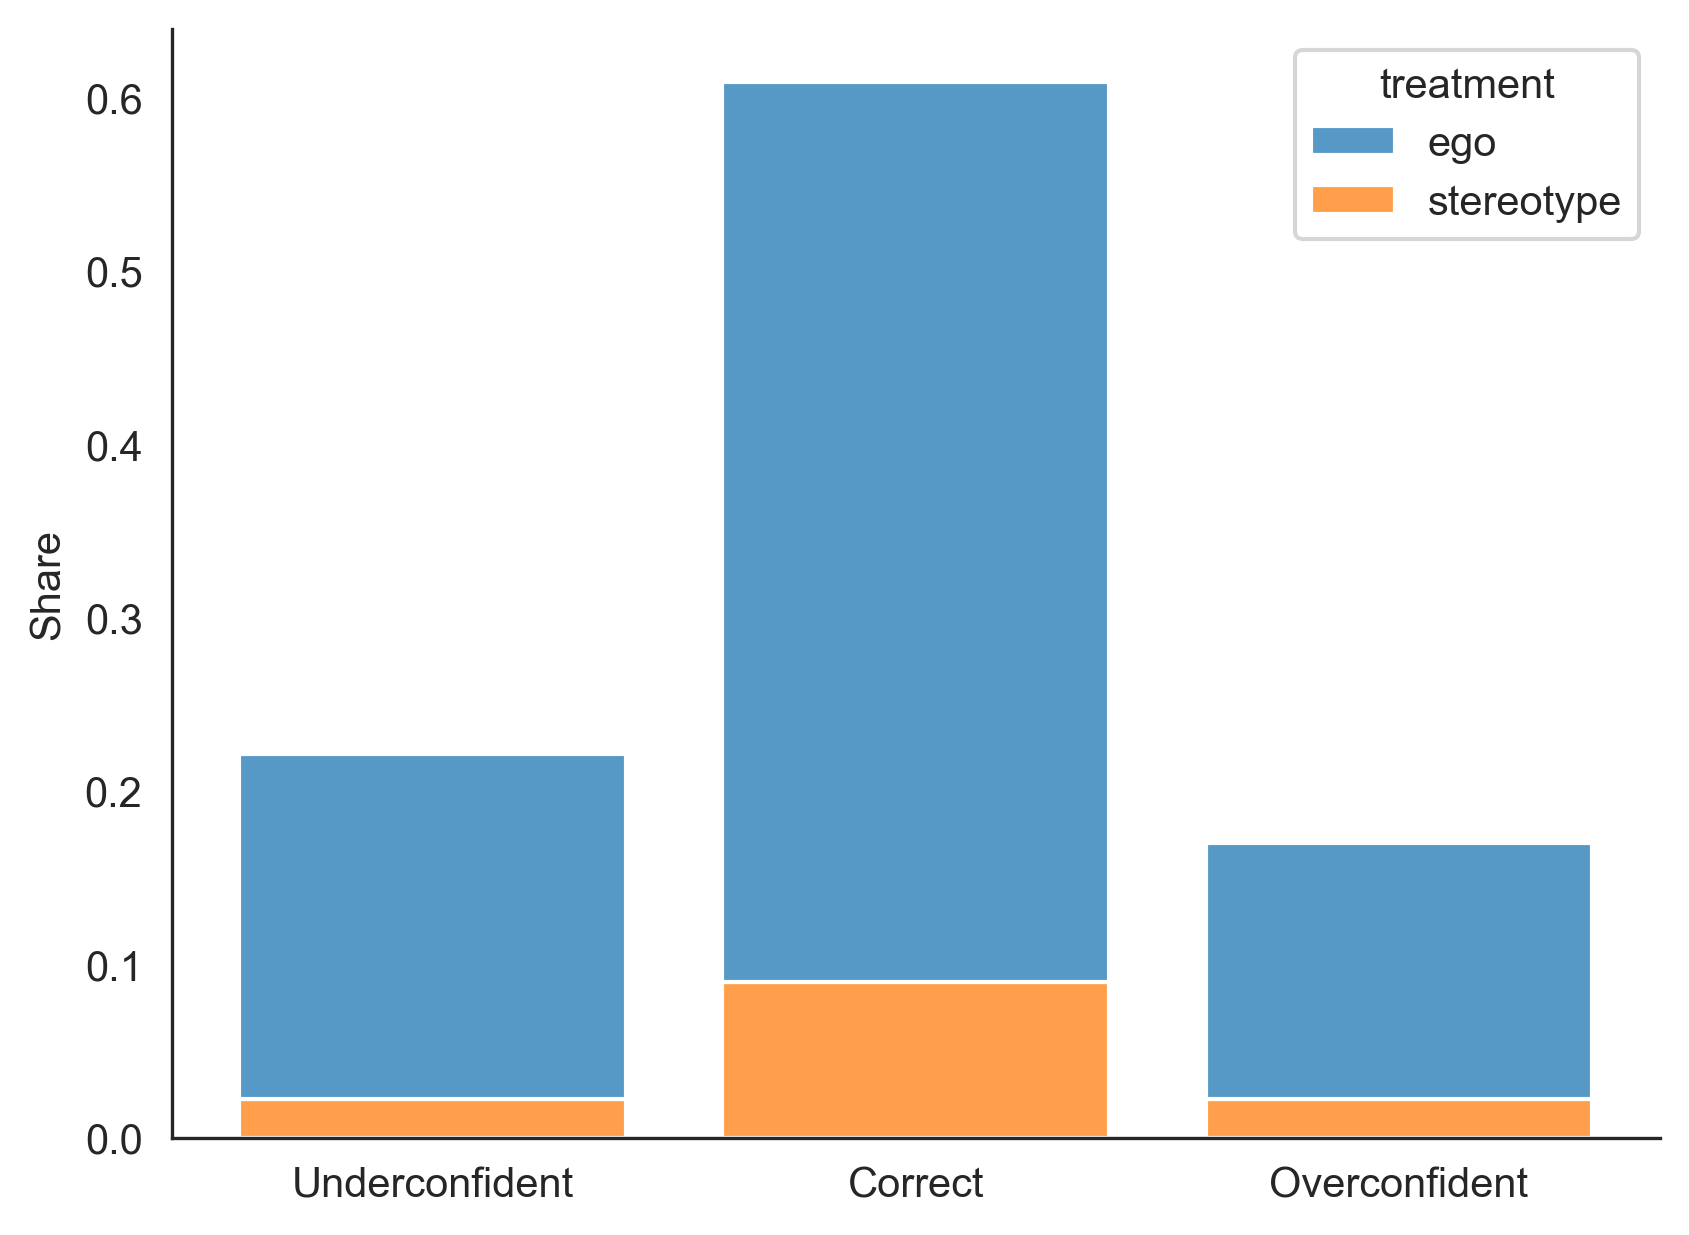
\includegraphics{../figures/misspecification_hist.png}
\caption{Initial misspecifications by
treatment}\label{fig:misspecification-hist}
}
\end{figure}

Although the overall distribution is similar for both treatments, the
misspecifications arise for different combinations of characteristics in
each treatment. Figure \ref{fig:misspecification-by-treatment} shows a
heatmap of the misspecifications that arose in each treatment. In the
stereotype treatment, subjects are most underconfident about the
performance of other non-American females in Sports and Video Games. In
contrast, they are most overconfident about the performance of American
men in Verbal Reasoning. In the ego-relevant treatment, subjects are
most underconfident about their own performance in pop culture and art,
while most overconfident about their performance in Verbal Reasoning.

\begin{figure}
\hypertarget{fig:misspecification-by-treatment}{%
\centering
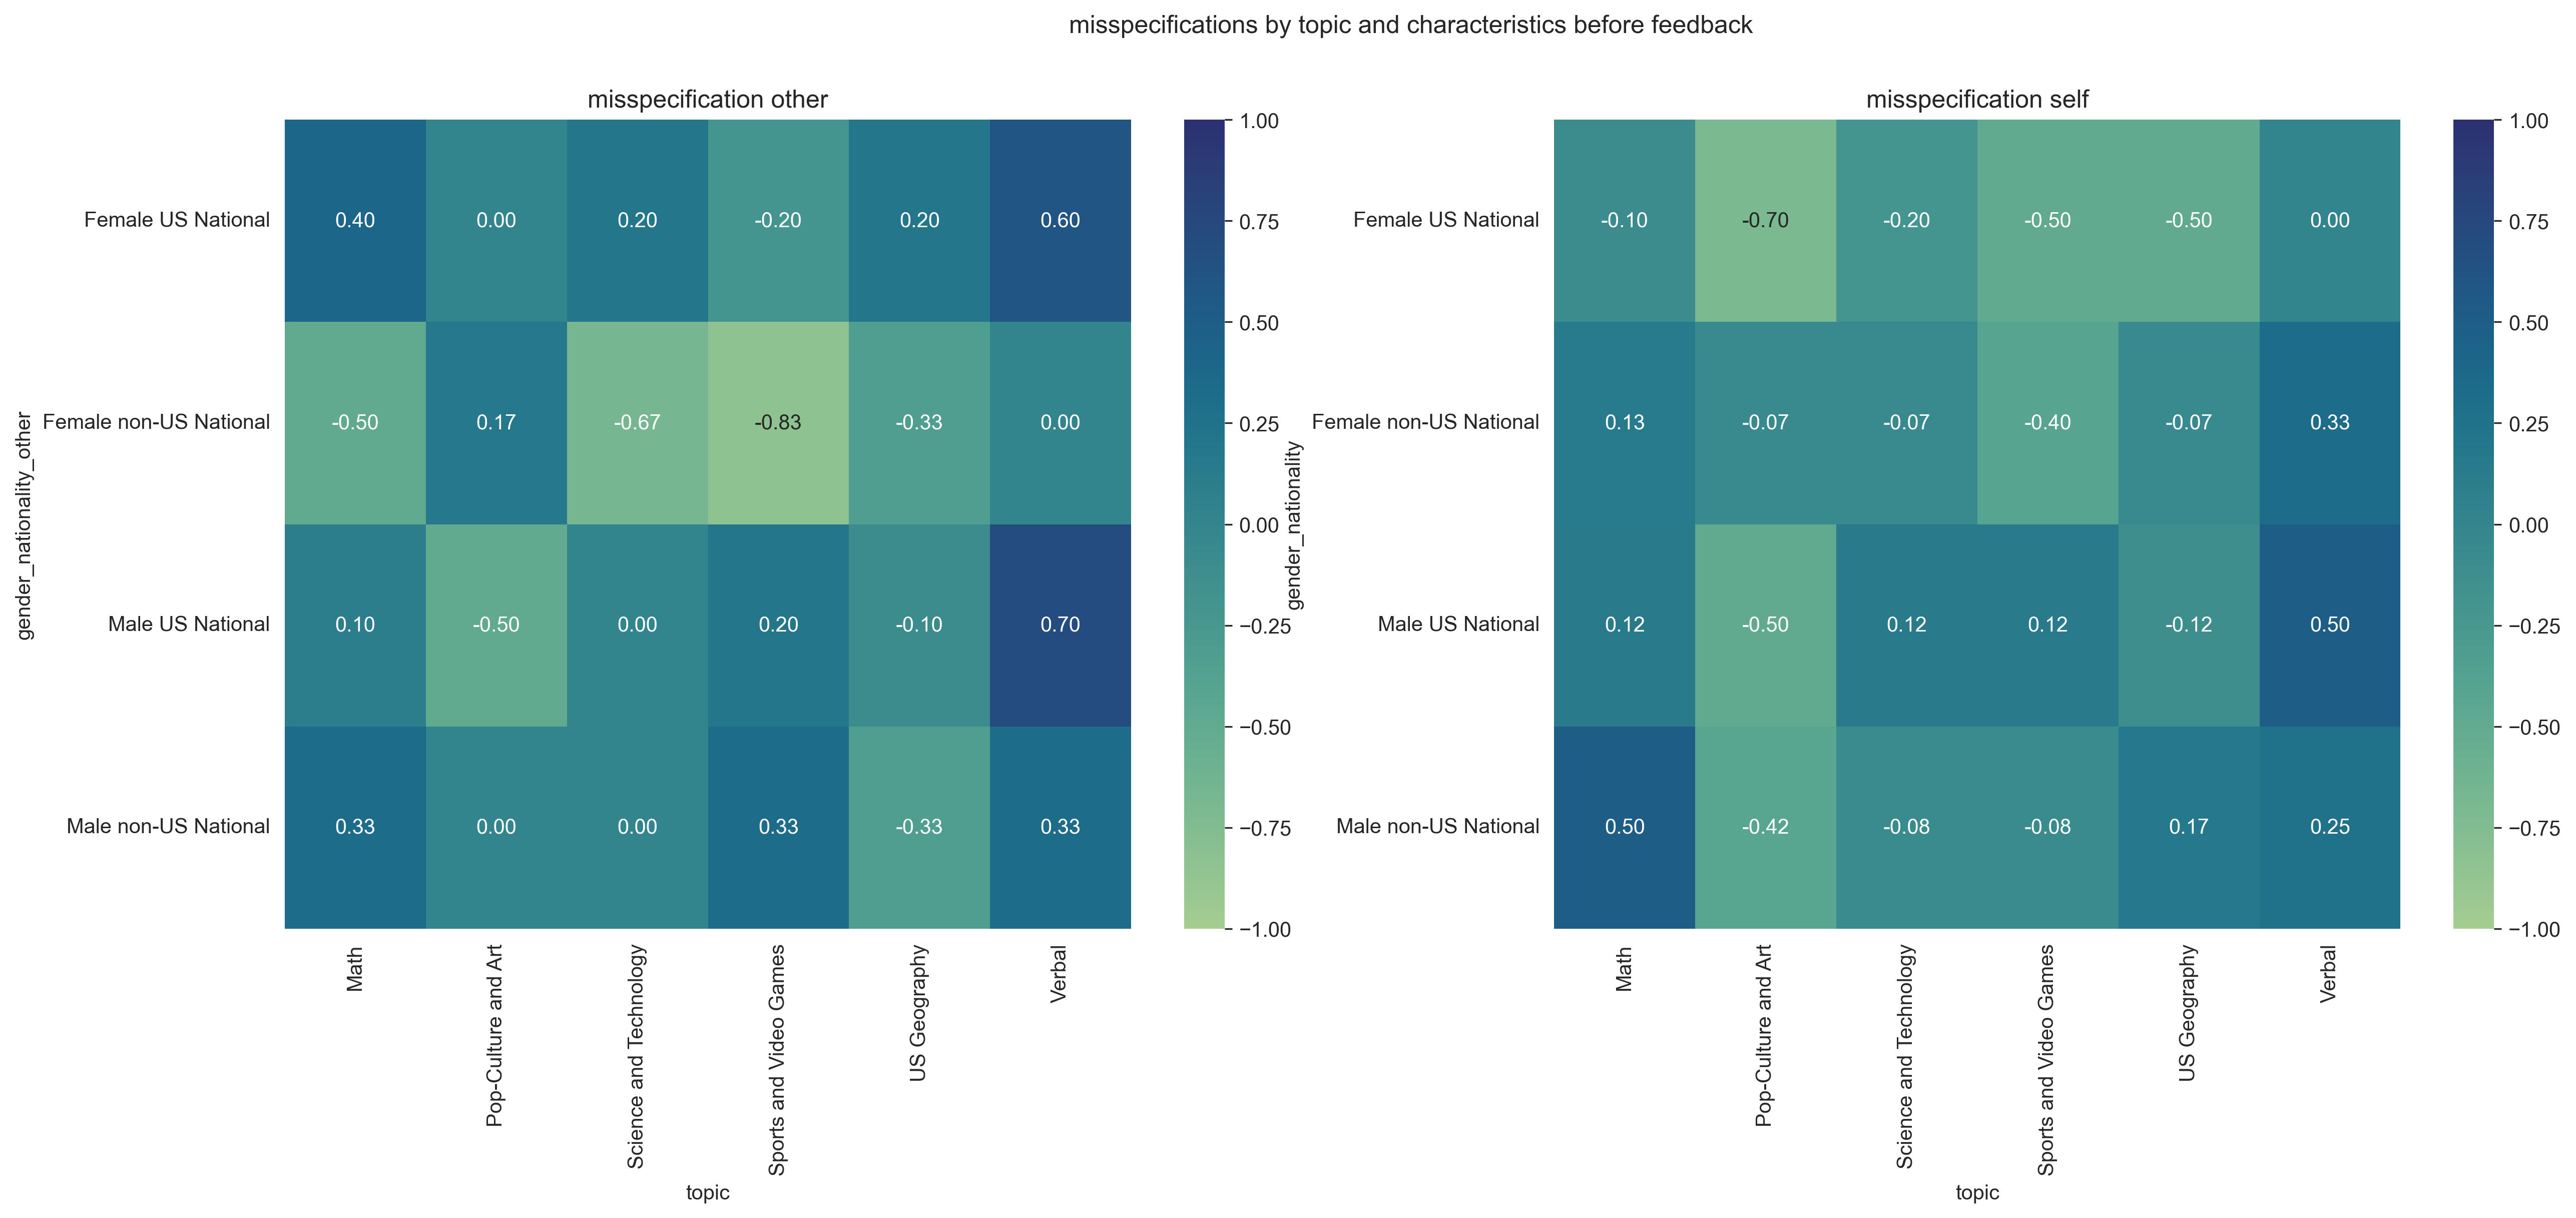
\includegraphics{../figures/misspecifications_characteristics_treatment.png}
\caption{Initial misspecifications by treatment and
characteristics}\label{fig:misspecification-by-treatment}
}
\end{figure}

Having widespread misspecifications in both treatments is important for
the analysis because it allows me to distinguish between the dogmatic
modeler and the switcher. If there were no misspecifications, the two
models would be indistinguishable.

\hypertarget{learning}{%
\subsection{Learning}\label{learning}}

In this section, I analyze the learning behavior of subjects in the
experiment. There are two parameters that subjects can be learning
about: the exogenous parameter \(\omega\) and the type \(\theta\). Their
belief about the exogenous parameter is tracked by their choice of
effort, while their belief about the type is tracked by their choice of
a matrix in which to enter their effort.

\hypertarget{learning-about-the-state}{%
\subsubsection{Learning about the
state}\label{learning-about-the-state}}

In order to analyze the learning about the state, I look at the share of
optimal choices that are made at each round. I find that although
subjects seem to be improving in their choices overall, the last choice
coincided with the true state only in 52\% of the choices in the last
round of each task. This is statistically greater than the initial share
of optimal choices of 30\% (\(p<0.01\)). However, it is still far from
complete learning. It is also important to note that learning is similar
across treatments. The share of choices that were consistent with the
true state for each round is reported in Figure
\ref{fig:optimal-choices-by-round}.

\begin{figure}
\hypertarget{fig:optimal-choices-by-round}{%
\centering
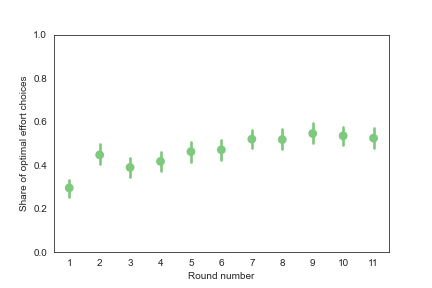
\includegraphics{../figures/effort_learning.png}
\caption{Share of optimal choices by
round}\label{fig:optimal-choices-by-round}
}
\end{figure}

A closer look at whether people learned or not reveals that there is a
good amount of heterogeneity in the sample. Figure
\ref{fig:learning-by-groups} shows the share of optimal choices by round
for subjects that chose an effort that matched the state in 3 out of the
last 4 rounds. It also shows the share of optimal choices for subjects
who chose an effort that matched the state in fewer than 3 out of the
last 4 rounds. I label the former as learners and the latter as
non-learners, with learners making up 0\% of the sample.

\begin{figure}
\hypertarget{fig:learning-by-groups}{%
\centering
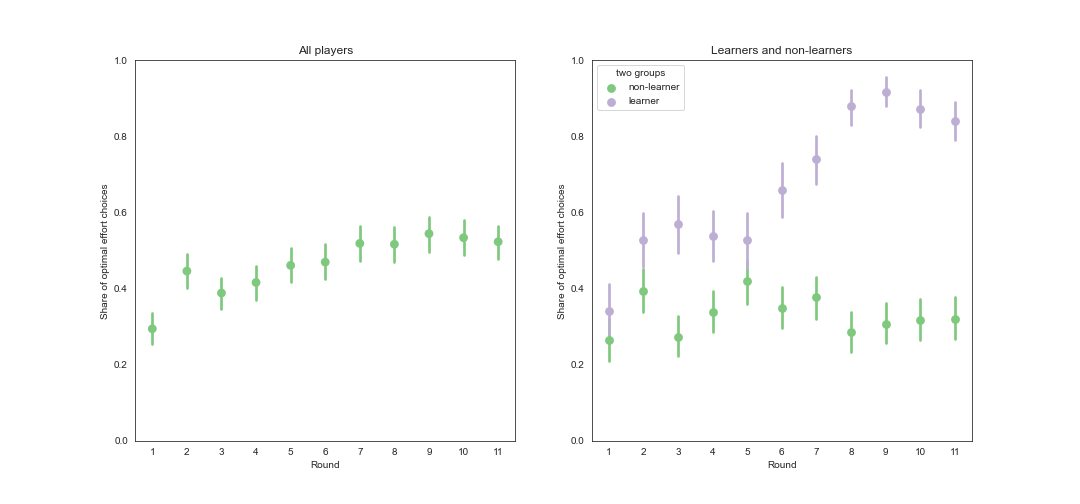
\includegraphics{../figures/learning_groups.png}
\caption{Share of optimal choices by round for subjects who learned
(their effort in at least 3 out of tha last 4 choices matched the
state), and subjects who did not learn}\label{fig:learning-by-groups}
}
\end{figure}

In what follows I will try to disentangle the reasons for the lack of
learning. I will argue that it is not due to the presence of traps, but
rather due to biased updating. According to the theories, the main
reason why subjects might not learn is that they have an incorrect
belief about the type or they develop an incorrect belief about the
type.

\hypertarget{learning-about-the-type}{%
\subsubsection{Learning about the type}\label{learning-about-the-type}}

\begin{figure}
\hypertarget{fig:matrix-choices-by-round}{%
\centering
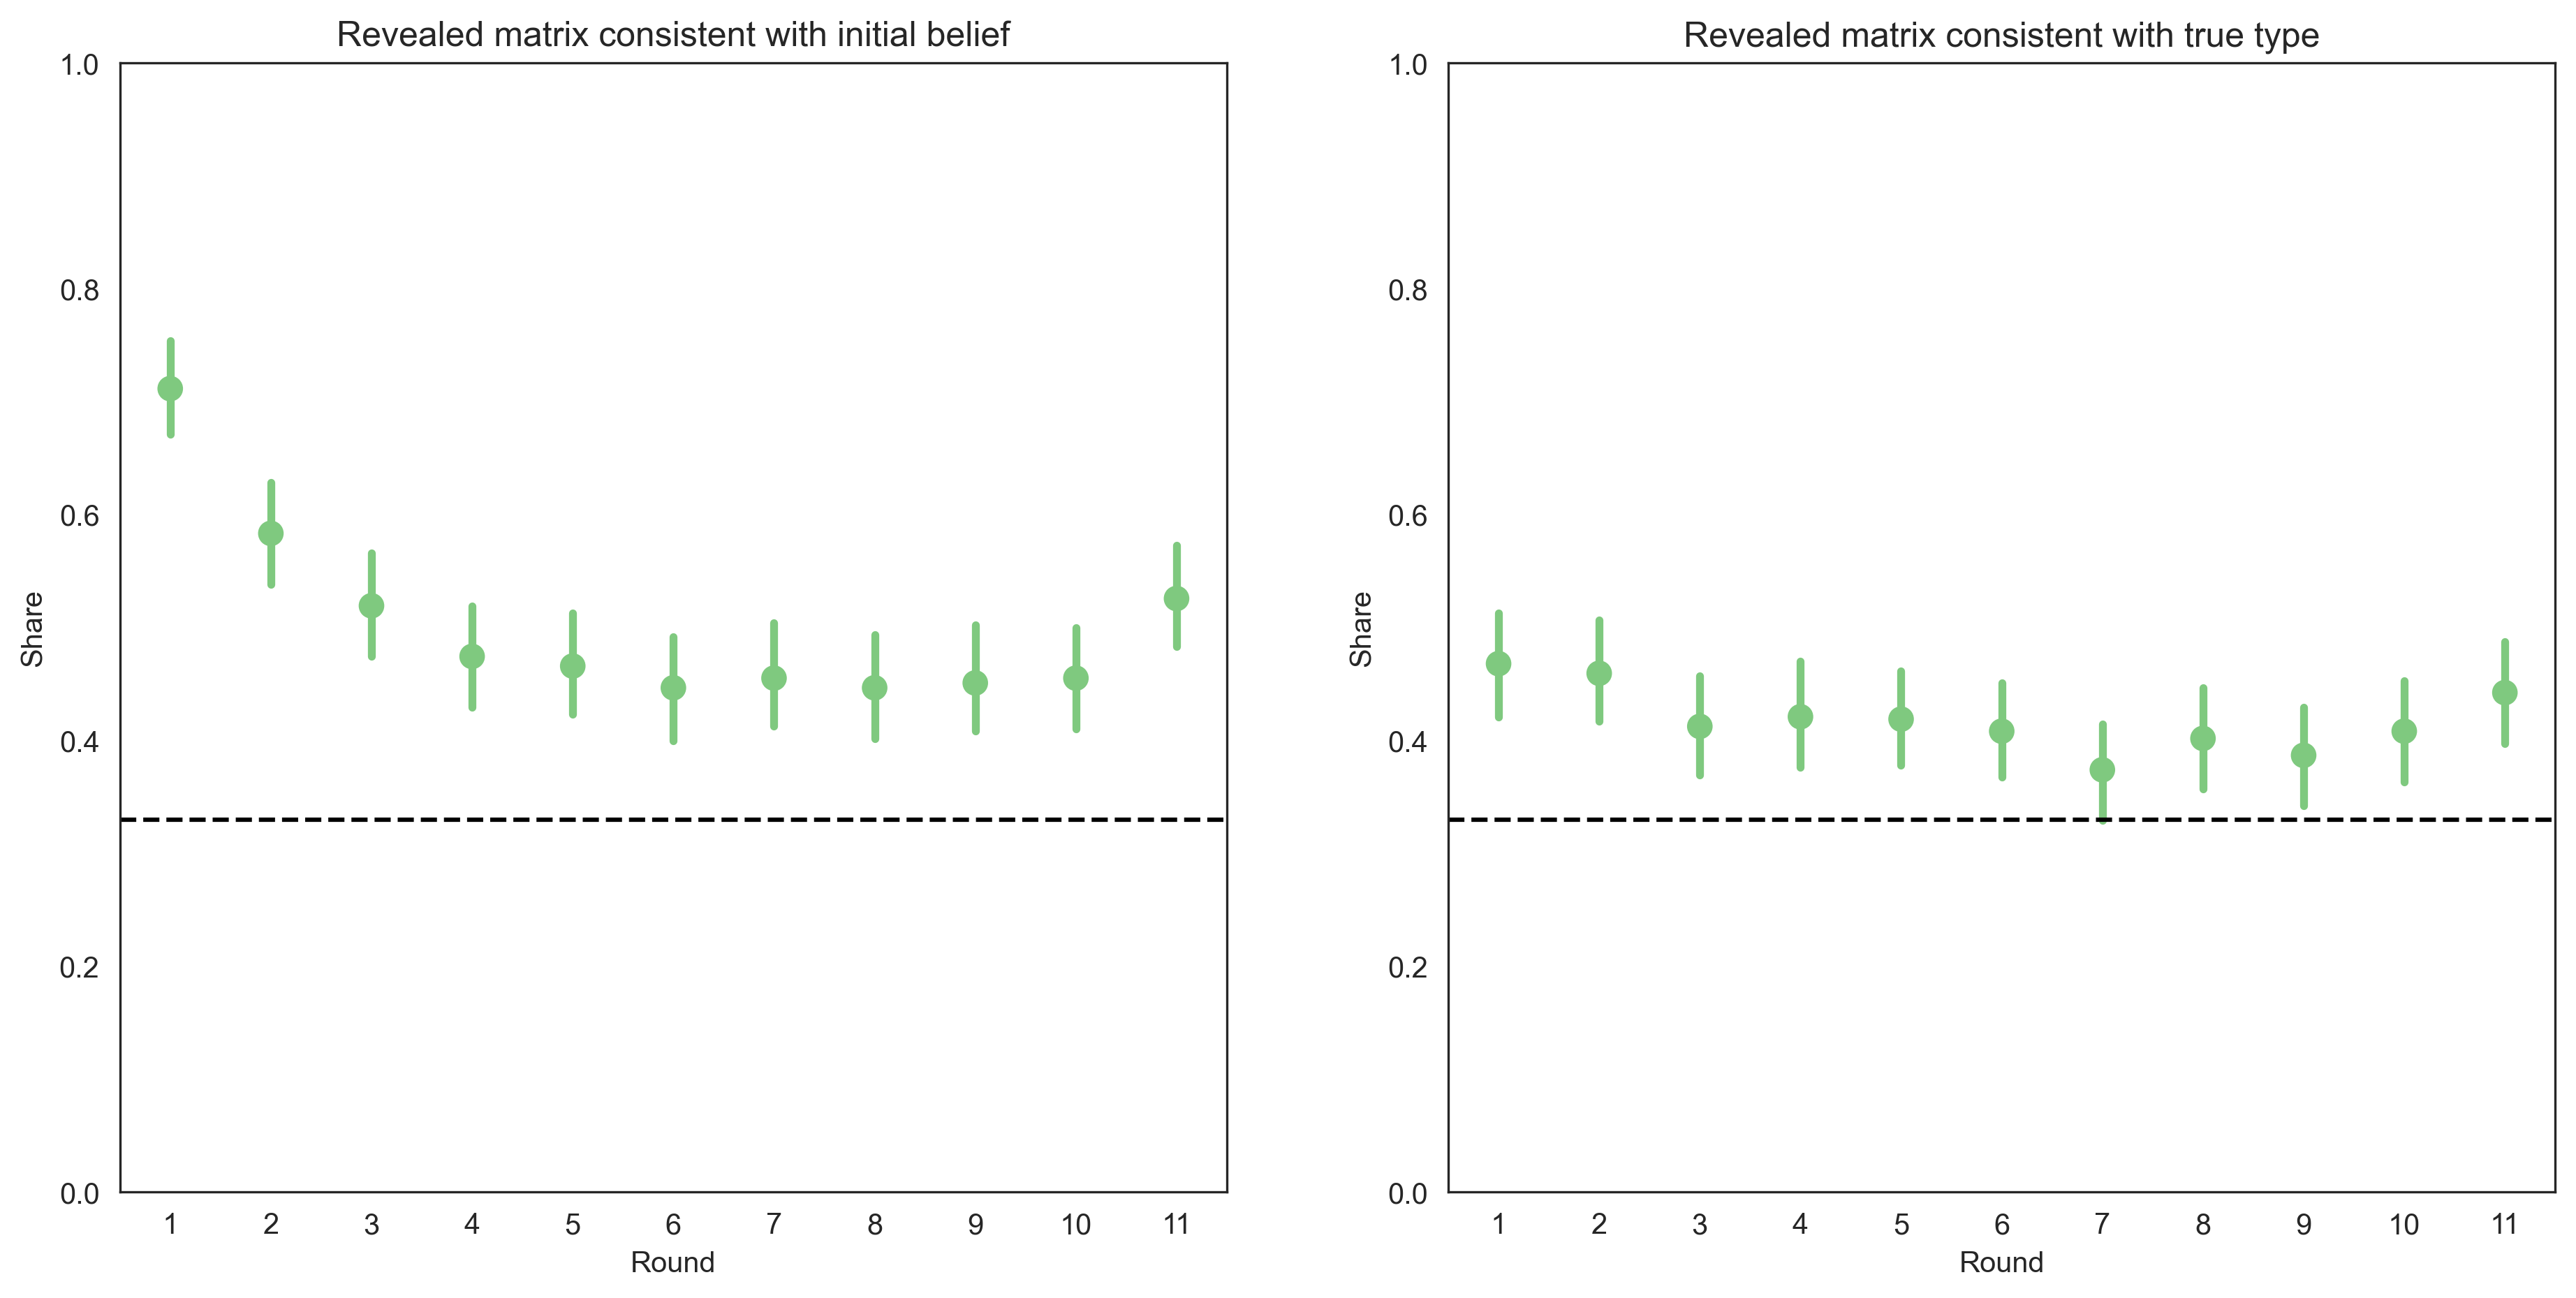
\includegraphics{../figures/last_button_consistency.png}
\caption{Matrix choices by round}\label{fig:matrix-choices-by-round}
}
\end{figure}

Since the elicitation of the belief about the type was not incentivized
and not elicited in a standard way, I first need to confirm that
subjects were not just randomly choosing a matrix in which to enter
their effort. The left panel of Figure \ref{fig:matrix-choices-by-round}
shows the share of subjects who chose a matrix consistent with their
initial reported belief. In round 1, 71\% of the subjects chose a matrix
that was consistent with their initial belief. This indicates that
subjects were not just randomly choosing a matrix in which to enter
their effort. From round 2 onwards, the share steadily declines, but
still not as far as to indicate a random choice of matrices. This is
consistent with the subjects moving away from their starting belief
through some updating procedure.

On the right panel of Figure \ref{fig:matrix-choices-by-round} I show
the share of subjects who chose a matrix that is consistent with their
true type. Unlike the left panel, there is no clear trend, which
indicates that although they are moving away from their initial belief,
they are not moving towards their true type, which means that overall,
misspecification is not decreasing. A closer look at the data reveals a
good amount of heterogeneity in the underlying behavior.

Figure \ref{fig:transitions} shows the transition matrix for subjects
who started in each of the 3 possible starting specifications and the
specifications that they ended up in at the end of the updating task.
The two things to note are that the initial belief is the most likely
end belief. This is consistent with some degree of stickiness of the
misspecifications as the switcher and dogmatic models would predict.
However, the data also presents a lot of subjects who started with a
correct belief of the type and ended up overestimating it. This is
consistent only with the self-attribution bias. Lastly, the subjects who
initially overestimate the score, are the least likely to learn their
true type.

\begin{figure}
\hypertarget{fig:transitions}{%
\centering
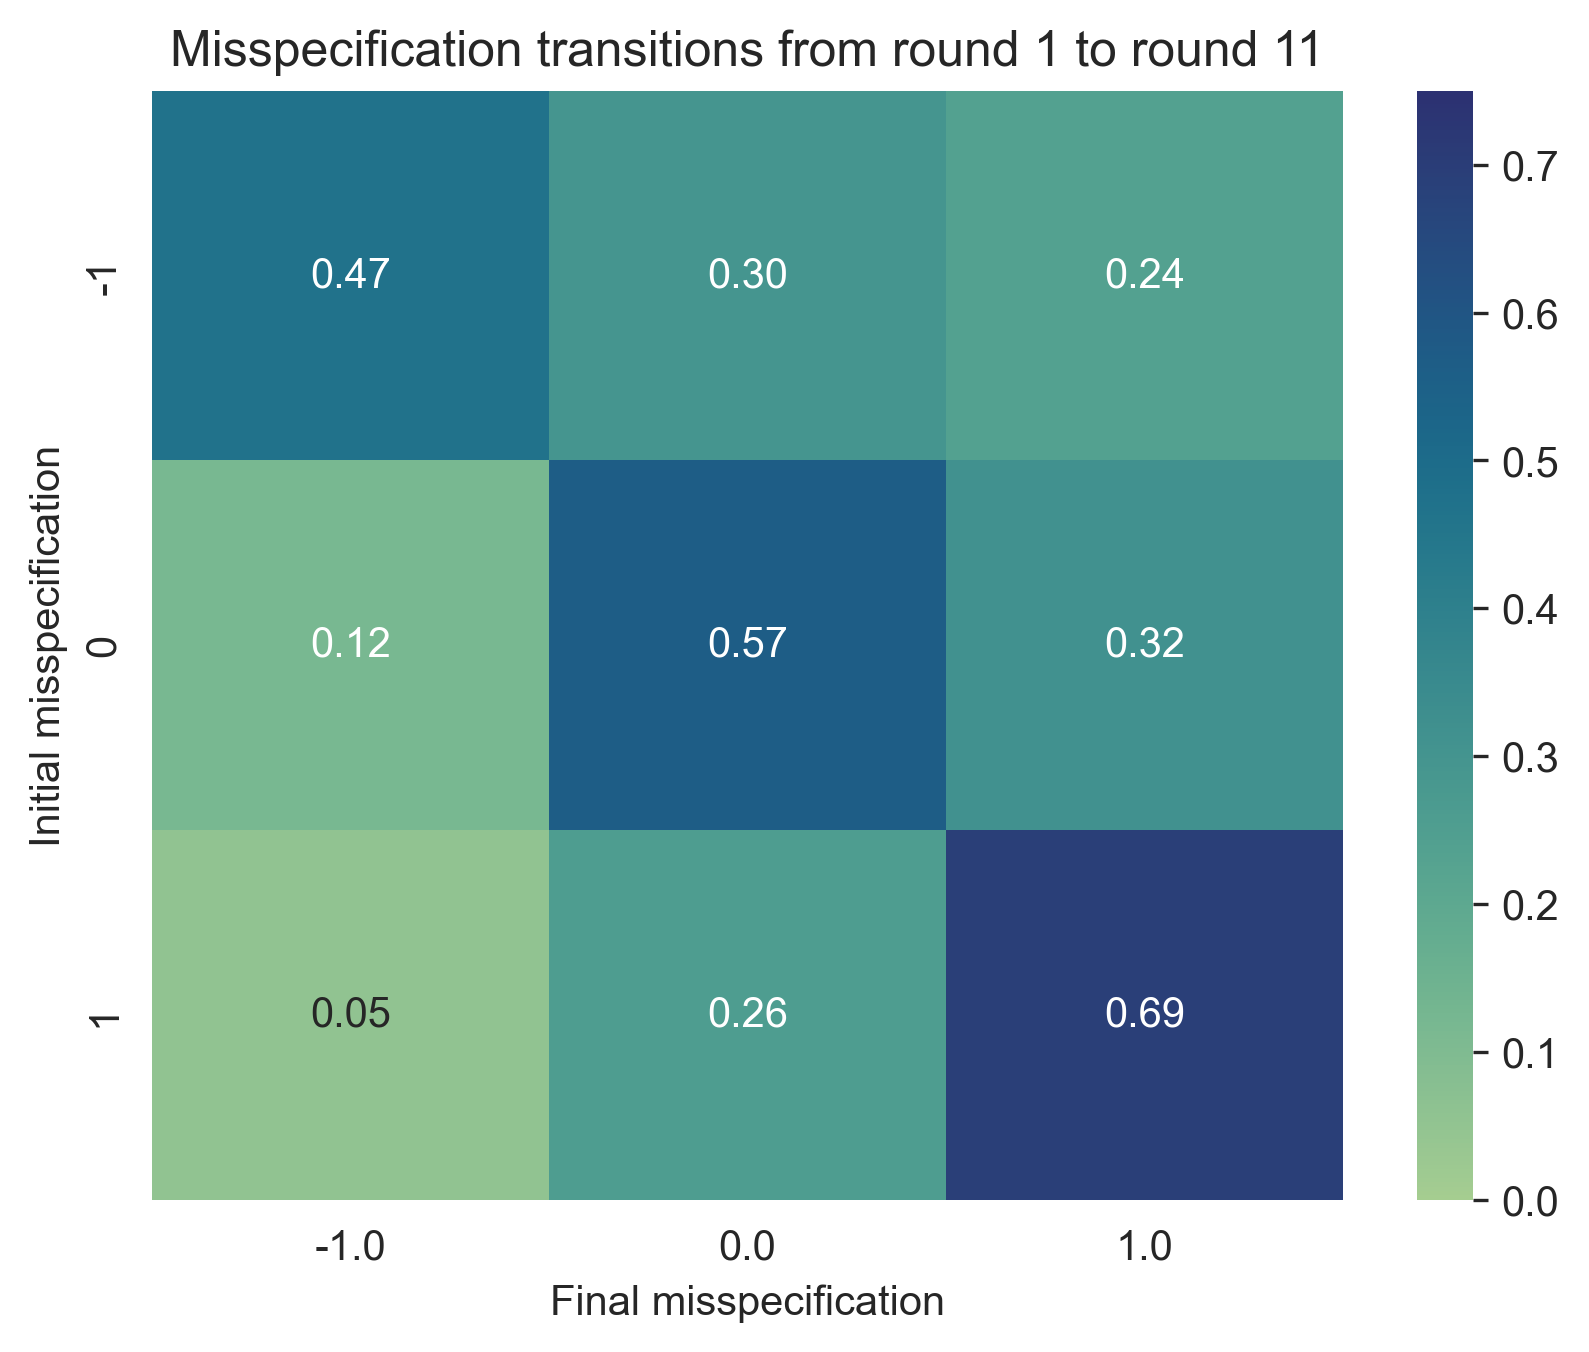
\includegraphics{../figures/misspecification_transitions.png}
\caption{Transition matrix for subjects who started in each of the 3
possible starting specifications and the specification that they ended
up in at the end of the updating task}\label{fig:transitions}
}
\end{figure}

This transition matrix

\hypertarget{reactions-to-good-and-bad-news}{%
\subsection{Reactions to good and bad
news}\label{reactions-to-good-and-bad-news}}

\hypertarget{conclusion}{%
\section{Conclusion}\label{conclusion}}

\renewcommand\refname{References}
  \bibliography{references.bib}

\end{document}
